\chapter{Конструкторский раздел}

В данном разделе будет спроектированы база данных и приложение для доступа к ней.

\section{Проектирование базы данных}

\subsection{Описание таблиц базы данных}
В базе данных библиотечной системы 7 таблиц. 

Таблица \texttt{Library} описывает основную информацию о библиотеках. Её поля:

Поля таблицы \texttt{Library}:
\begin{itemize}
	\item \texttt{id} -- идентификатор библиотеки (целое);
	\item \texttt{name} -- название библиотеки (строка);
	\item \texttt{address} -- автор библиотеки (строка).
\end{itemize}

Таблица \texttt{Account} описывает основную информацию о библиотеках. Её поля:

Поля таблицы \texttt{Account}:
\begin{itemize}
	\item \texttt{id} -- идентификатор аккаунта (целое);
	\item \texttt{login} -- логин пользователя (строка, уникальный);
	\item \texttt{password} -- пароль пользователя (строка);
	\item \texttt{name} -- имя пользователя (строка);
	\item \texttt{role} -- роль пользователя в системе (администратор, библиотекарь, читатель) (строка).
\end{itemize}

Таблица \texttt{Book} описывает основную информацию о книгах. Её поля:
\begin{itemize}
	\item \texttt{id} -- идентификатор книги (целое);
	\item \texttt{name} -- название книги (строка);
	\item \texttt{author} -- автор книги (строка).
\end{itemize}

Таблица \texttt{BookItem} описывает экземпляр книги. Данная таблица реализует 3 связи 1 ко многим. Её поля:
\begin{itemize}
	\item \texttt{id} -- идентификатор экземпляра книги (целое);
	\item \texttt{bokk\_id} -- идентификатор дескриптора книги (целое);
	\item \texttt{lib\_id} -- идентификатор библиотеки, в которой хранится экземпляр книги (целое);
	\item \texttt{acc\_id} -- идентификатор аккаунта читателя (целое или пустое, если книга в библиотеке).
\end{itemize}

Таблица \texttt{Librarian} описывает сущность библиотекаря. Её поля:
\begin{itemize}
	\item \texttt{id} -- идентификатор аккаунта библиотекаря (целое);
	\item \texttt{lib\_id} -- идентификатор библиотеки, в которой работает библиотекарь (целое).
\end{itemize}

Таблица \texttt{Administrator} описывает сущность администратора. Её поля:
\begin{itemize}
	\item \texttt{id} -- идентификатор аккаунта администратора (целое).
\end{itemize}

Таблица \texttt{Librarian} описывает сущность читателя. Её поля:
\begin{itemize}
	\item \texttt{id} -- идентификатор аккаунта читателя (целое);
	\item \texttt{lib\_id} -- телефон читателя (строка).
\end{itemize}
\newpage
\subsection{Описание функций базы данных}
Кроме того, в базе данных определены 2 функции:
\begin{enumerate}
    \item Функция взятия книги в библиотеке, состоящая из следующих действий: по логину библиотекаря вычисляется идентификатор библиотеки, в которой библиотекарь имеет возможность выдавать книги; вычисляется идентификатор читателя по логину читателя; идентификатор читателя ставится в поле \texttt{acc\_id} экземпляру книги, находящемуся в данной библиотеке. 
    \item Функция возврата книги в библиотеку, состоящая из следующих действий: по логину библиотекаря вычисляется идентификатор библиотеки, в которой библиотекарь имеет возможность выдавать книги; вычисляется идентификатор читателя по логину читателя; поле \texttt{acc\_id} становится пустым у того экземпляра книги, который находится в данной библиотеке и взят читателем с найденным идентификатором. 
\end{enumerate}

На рисунке \ref{fig:funcs} представлены схемы алгоритмов описанных функций.

\begin{figure}[H]
	\centering
	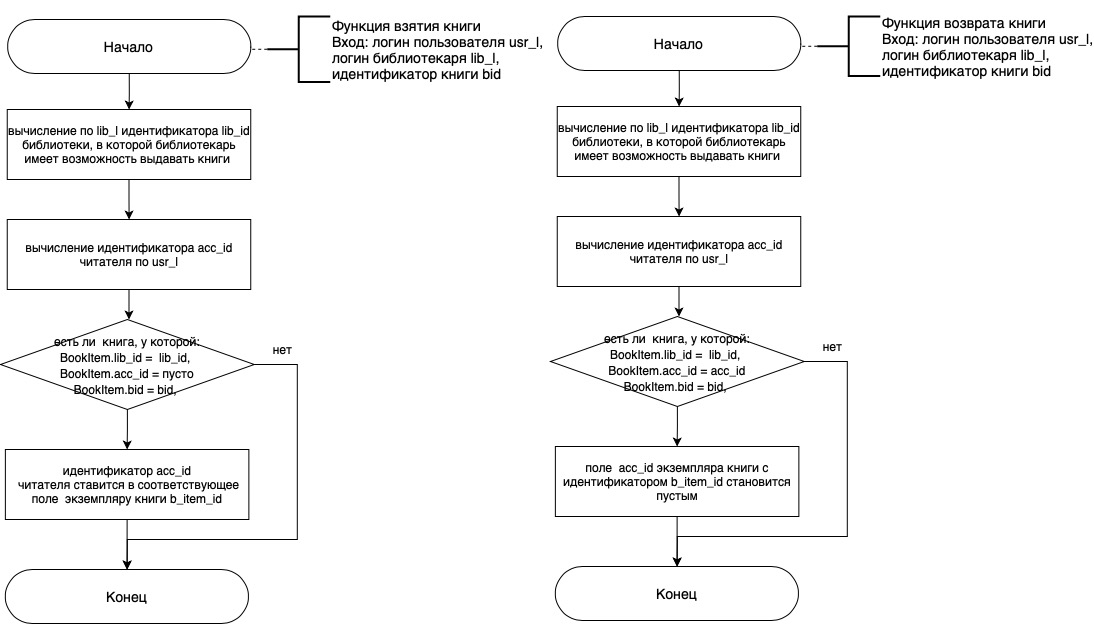
\includegraphics[width = \linewidth]{img/funcs_triggers-funcs.jpg}
	\caption{Схемы функций базы данных}
	\label{fig:funcs}
\end{figure}

\subsection{Описание триггеров базы данных}

Также для поддержания логической непротиворечивости базы данных определено 2 триггера:
\begin{enumerate}
    \item \texttt{DML-триггер before delete}, определённый на таблице \texttt{Account}. До \\удаления аккаунта все книги, взятые пользователем, принудительно возвращаются в бибиотеку.
    \item \texttt{DML-триггер before delete}, определённый на таблице \texttt{Library}. До \\удаления все аккаунты библиотекарей, работающих в данной библиотеке, удаляются.
\end{enumerate}

На рисунке \ref{fig:triggers} представлены схемы алгоритмов описанных триггеров.

\begin{figure}[H]
	\centering
	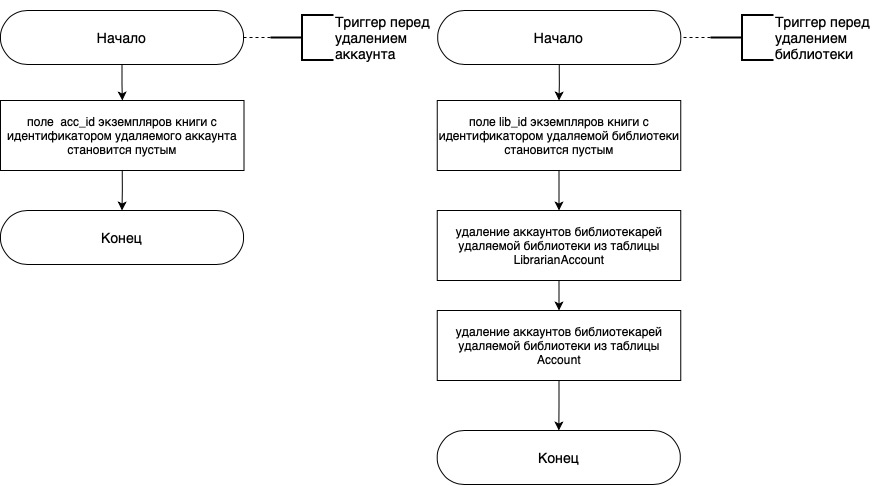
\includegraphics[width = \linewidth]{img/funcs_triggers-triggers.jpg}
	\caption{Схемы триггеров базы данных}
	\label{fig:triggers}
\end{figure}
\newpage
\subsection{Описание транзакций базы данных}
Для поддержания целостности базы данных используются следующие \\транзакции:
\begin{enumerate}
    \item при добавлении книги проверяется, есть ли уже книга с таким названием и автором; если есть, то добавляется экземпляр книги и возвращается его идентификатор; если нет, то обновляются две таблицы: дескрипторов книг и экземпляров книг, возвращается идентификатор экземпляра;
    \item при изменении книги проверяется, существует ли библиотека с указанным идентификатором; если существует, то обновляются дескриптор книги (обновляются все поля, кроме идентификатора) и экземпляр книги (меняется идентификатор библиотеки);  если нет, то происходит откат;
    \item при добавлении, удалении и изменении аккаунта обновляются 2 таблицы: таблица аккаунтов и таблица, соответсвующая роли; кроме того, при добавлении и изменении аккаунта библиотекаря проверяется, существует ли библиотека с указанным идентификатором;
\end{enumerate}

\subsection{Ролевая модель}
Для безопасной работы с данными вводится 3 типа пользователей:
\begin{enumerate}
    \item администраторы, которые имеют полный доступ ко всем объектам базы данных;
    \item библиотекари, которые имеют права на обновление таблицы экземпляров книг и на чтение всех остальных таблиц;
    \item читатели, которые имеют права только на чтение всех таблиц.
\end{enumerate}

\section{Проектирование приложения}
Для реализации поставленной задачи наиболее подходящей является кли- ент-серверная архитектура, так как она позволяет нескольким клиентам работать одновременно с приложением. Таким образом, приложение должно состоять из 3 основных компонентов:
\begin{itemize}
    \item компонент доступа к данным, который реализует обращение к базе данных и предоставляет интерфейс в виде доступных команд;
    \item компонент бизнес-логики, который занимается диспетчеризацией поступающих запросов соответствующим командам компонента доступа к данным;
    \item компонент интерфейса, который обращается к компоненту бизнес-логи- ки за данными и занимается их отображением.
\end{itemize}
Связь компонентов показана на рисунке \ref{fig:comps}.
\begin{figure}[H]
	\centering
	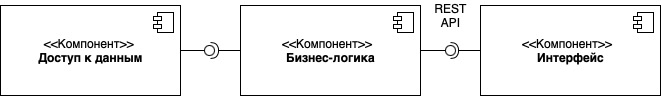
\includegraphics[width = \linewidth]{img/components.jpg}
	\caption{Схема компонентов приложения}
	\label{fig:comps}
\end{figure}

\section*{Вывод}
\addcontentsline{toc}{section}{Вывод}

В данном разделе в качестве архитектуры приложения была выбрана клиент-серверная архитектура и приведена схема компонентов для её реализации. Кроме того, была спроектирована база данных: описаны её триггеры, функции, сущности и связи между ними, а также транзакции.
